\usetikzlibrary{shadows,shapes.multipart}

\title{Endianness}


\begin{document}

\begin{frame}
  \titlepage
\end{frame}

\section{Decimal Notation}

\begin{frame}
  \frametitle{Decimal Notation}
  \begin{itemize}
    \item Number is split up in digits
    \item Each digit has its own weight
    \item Digits ordered in \emph{decreasing} order of significance
  \end{itemize}
  \vskip5mm
  \begin{center}
    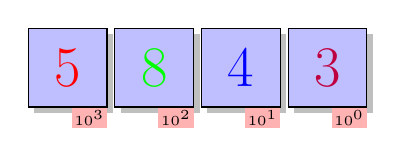
\begin{tikzpicture}[digit/.style={draw,minimum size=1cm,font=\huge,fill=blue!25,drop shadow},
                        weight/.style={font=\tiny,fill=red!30,inner sep=1pt}]
      \foreach[count=\i,evaluate={(\i-1)*1.1} as \x] \d/\c in {5/red,8/green,4/blue,3/purple} {
        \node[digit] (d\i) at (\x,0) {\color{\c} \d};
      }

      \node[weight,anchor=north east] at (d1.south east) { $10^3$ };
      \node[weight,anchor=north east] at (d2.south east) { $10^2$ };
      \node[weight,anchor=north east] at (d3.south east) { $10^1$ };
      \node[weight,anchor=north east] at (d4.south east) { $10^0$ };
    \end{tikzpicture}
  \end{center}
  \[
    {\color{red} 5} \times 10^3 \;+\; {\color{green} 8} \times 10^2 \;+\; {\color{blue} 4} \times 10^1 \;+\; {\color{purple} 3} \times 10^0
  \]
\end{frame}

\begin{frame}
  \frametitle{Alternative Decimal Notation}
  \begin{itemize}
    \item Order of digits is arbitrary
    \item Why digit with largest weight first?
    \item Why not digit with lowest weight first?
  \end{itemize}
  \vskip5mm
  \begin{center}
    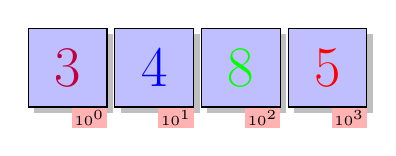
\begin{tikzpicture}[digit/.style={draw,minimum size=1cm,font=\huge,fill=blue!25,drop shadow},
                        weight/.style={font=\tiny,fill=red!30,inner sep=1pt}]
      \foreach[count=\i,evaluate={3.3-(\i-1)*1.1} as \x] \d/\c in {5/red,8/green,4/blue,3/purple} {
        \node[digit] (d\i) at (\x,0) {\color{\c} \d};
      }

      \node[weight,anchor=north east] at (d1.south east) { $10^3$ };
      \node[weight,anchor=north east] at (d2.south east) { $10^2$ };
      \node[weight,anchor=north east] at (d3.south east) { $10^1$ };
      \node[weight,anchor=north east] at (d4.south east) { $10^0$ };
    \end{tikzpicture}
  \end{center}
  \[
    {\color{purple} 3} \times 10^0 \;+\;
    {\color{blue} 4} \times 10^1 \;+\;
    {\color{green} 8} \times 10^2 \;+\;
    {\color{red} 5} \times 10^3
  \]
\end{frame}

\begin{frame}
  \frametitle{Endianness}
  \begin{itemize}
    \item Endianness: order in which digits are placed
    \item Little endian: least significant digits first
    \item Big endian: most significant digits first
    \item Our decimal system is big endian
  \end{itemize}
\end{frame}

\begin{frame}
  \frametitle{Examples}
  \begin{itemize}
    \item Dates are little endian: day $<$ month $<$ year
          \begin{center}
            \begin{tikzpicture}[digit/.style={draw,minimum size=1cm,fill=blue!25,drop shadow}]
              \node[digit,anchor=base] (d1) at (0,0) {day};
              \node[digit,anchor=west] (d2) at ($ (d1.east) + (0.1,0) $) {month};
              \node[digit,anchor=west] (d3) at ($ (d2.east) + (0.1,0) $) {year};
            \end{tikzpicture}
          \end{center}
    \item Time is big endian: hours $>$ minutes $>$ seconds
          \begin{center}
            \begin{tikzpicture}[digit/.style={draw,minimum size=1cm,fill=blue!25,drop shadow}]
              \node[digit,anchor=base] (d1) at (0,0) {hours};
              \node[digit,anchor=west] (d2) at ($ (d1.east) + (0.1,0) $) {minutes};
              \node[digit,anchor=west] (d3) at ($ (d2.east) + (0.1,0) $) {seconds};
            \end{tikzpicture}
          \end{center}
  \end{itemize}
\end{frame}

\begin{frame}
  \frametitle{Endianness in Computing}
  \begin{itemize}
    \item Endianness also applies on computer architectures
    \item But how exactly does it apply?
  \end{itemize}
  \begin{overprint}
    \onslide<1|handout:1>
    \structure{On the level of bits?}
    \begin{center}
      \begin{tikzpicture}[digit/.style={draw,minimum size=1cm,fill=blue!25,drop shadow}]
        \foreach[count=\i,evaluate={(\i-1)*1.1} as \x] \d in {1,0,0,1,1,1,0,0} {
          \node[digit] (d\i) at (\x,0) {\d};
        }

        \node at ($ (3.3, 1) ! 0.5 ! (4.4,1) $) {vs};

        \foreach[count=\i,evaluate={7.7-(\i-1)*1.1} as \x] \d in {1,0,0,1,1,1,0,0} {
          \node[digit] (d\i) at (\x,2) {\d};
        }
      \end{tikzpicture}
    \end{center}

    \onslide<2|handout:2>
    \structure{On the level of hexadecimal digits?}
    \begin{center}
      \begin{tikzpicture}[digit/.style={draw,minimum size=1cm,fill=blue!25,drop shadow,font=\small}]
        \foreach[count=\i,evaluate={(\i-1)*1.1} as \x] \d in {0x1,0xA,0x3,0x7} {
          \node[digit] (d\i) at (\x,0) {\d};
        }

        \node at ($ (1.1, 1) ! 0.5 ! (2.2,1) $) {vs};

        \foreach[count=\i,evaluate={3.3-(\i-1)*1.1} as \x] \d in {0x1,0xA,0x3,0x7} {
          \node[digit] (d\i) at (\x,2) {\d};
        }
      \end{tikzpicture}
    \end{center}

    \onslide<3|handout:3>
    \structure{On the level of bytes?}
    \begin{center}
      \begin{tikzpicture}[digit/.style={draw,minimum size=1cm,fill=blue!25,drop shadow,font=\small}]
        \foreach[count=\i,evaluate={(\i-1)*1.1} as \x] \d in {0x15,0x9A,0x13,0x45} {
          \node[digit] (d\i) at (\x,0) {\d};
        }

        \node at ($ (1.1, 1) ! 0.5 ! (2.2,1) $) {vs};

        \foreach[count=\i,evaluate={3.3-(\i-1)*1.1} as \x] \d in {0x15,0x9A,0x13,0x45} {
          \node[digit] (d\i) at (\x,2) {\d};
        }
      \end{tikzpicture}
    \end{center}
  \end{overprint}
\end{frame}

\begin{frame}
  \frametitle{x86/x64 Architecture}
  \begin{itemize}
    \item Endianness operates on \emph{level of bytes}
    \item Take good look at this!
  \end{itemize}
  \code[language=c++14]{i32.cpp}
  \begin{center}
    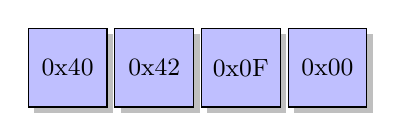
\begin{tikzpicture}[digit/.style={draw,minimum size=1cm,fill=blue!25,drop shadow,font=\small}]
      \foreach[count=\i,evaluate={3.3-(\i-1)*1.1} as \x] \d in {0x00,0x0F,0x42,0x40} {
        \node[digit] (d\i) at (\x,2) {\d};
      }
    \end{tikzpicture}
  \end{center}
\end{frame}

\begin{frame}
  \frametitle{Determining How 32-bit Value Is Stored}
  \begin{itemize}
    \item Convert value to hexadecimal
    \item Pad with zeros to the left until 8 digits long
    \item Group bytes
          \begin{itemize}
            \item Reminder: 1 byte = 2 hexadecimal digits
          \end{itemize}
    \item Reverse order of bytes
  \end{itemize}
\end{frame}

\begin{frame}
  \frametitle{Example: How Is 123456789 Stored In RAM?}
    \structure{Step 1: Convert to hexadecimal}
    \begin{center} \ttfamily
      123456789 = 0x75BCD15
    \end{center}

    \structure{Step 2: Pad with zeros}
    \begin{center} \ttfamily
      0x75BCD15 $\rightarrow$ 0x075BCD15
    \end{center}

    \structure{Step 3: Group Bytes}
    \begin{center} \ttfamily
      0x075BCD15 $\rightarrow$ 0x07 0x5B 0xCD 0x15
    \end{center}

    \structure{Step 4: Reverse Order}
    \begin{center} \ttfamily
      0x07 0x5B 0xCD 0x15 $\rightarrow$ 0x15 0xCD 0x5B 0x07
    \end{center}
\end{frame}

\end{document}
